%
%
%
\chapter{Spin-Fermion-Model}
\label{ch:spin fermion model}
%
%
%
In the following chapter the spin-fermion-model for a metal exhibiting a antiferromagnetic quantum phase transition is introduced as presented in \cite{Abanov&Chubukov&Schmalian}.
Beside fermionic particle-hole-exitetaions in the vicinity of the quantum critical point bosonic spin fluctuations arise in this low energy theory, which enable a attractive interaction between electrons.
This chapter isn't displayed a detailed mathematical or microscopic derivation of the spin-fermion-model, but rather it is based on a qualitative description to justified its form.
For that a shortly overview over quantum phase transitions are established as suggested in \cite{SachdevQCP}.
In particular, we focus one's attention on the arising spin fluctuations, agrue them carry large momenta and introduced the damped spin density propagator and their perodicity.
Further we present the basic concepts of hot-spot theory, which are points on the Fermi surface in 2D emerged since the magnetic Brillouin zone cutting the Fermi surface.
Besides we review explicitly the conservation of momentum and non-conservation of current for the observing Hamiltonian.
For breaking translation symmetry umklapp scattering is introduced and we prove that this is unconserving momentum.
%
%
\section{The Spin-Fermion-Model at the Onset of the Antiferromagnetic Quantum Phase Transition}
\label{sec:spin-fermion-model}
%
%
Many metals exhibit an antiferromagnetic phase transition at a characteristic temperature $\mt{T}_{\mt{N}}$, called N\'eel-temperature.
The random ordered spins of lattice atoms ordering in consequence of thermal fluctuations along one axis, where the nearest neighbors are always aligned in opposite direction.
This temperature can be changed by tuning a certain parameter like pressure or doping, for example.
A schematic and simplified phase diagram is depicted in figure \ref{fig:phase diagram}.
%
\begin{figure}[t]
	\centering
	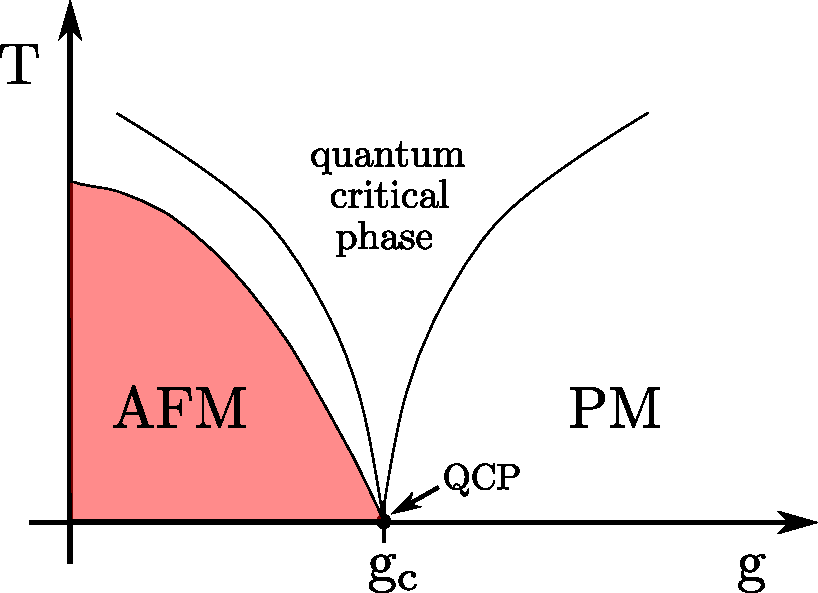
\includegraphics[width=0.7\textwidth]{phase_diagram.pdf}
	\caption{
This figure shows a schematic and simplified phase diagram for metals transition from a paramagnetic (PM) into an antiferrmagnetic (AFM) phase depending on a tunung parameter g.
The phase line of the AFM phase ends decreasing temperature down to $T = 0$ in a quantum critical point (QCP) at $\mt{g} = \mt{g}_{\mt{c}}$.
At this point the phase transition is only caused by quantum fluctuations.
At $T > 0$ thermal fluctuactions more and more dominates the phase transition.
Nevertheless quantum fluctuations influences the physical behaviour in a lagre regime, labeled as quantum critical phase.
	}
	\label{fig:phase diagram}
\end{figure}
%
Decreasing tempearutre the phase line between both magnetic phases reach a certain value for the tuning parameter g at $T = 0$, labeled with $\mt{g}_{\mt{c}}$.
This point is called quantum critical point and in comparsion with the phase transition at finite temperature quantum fluctuations are the origin of this phase transition.

Before starting with a qualitative derivation of the spin-fermion-model a short and rudimentary describtion of quantum phase transition is given.
This overview is required for the analytical discussion of our computation later.
However, the reason for phase transitions is always level crossing between the ground and an excited state.
Due to the fact that level crossing is forbidden a band gap $\Delta$ arises.
This band gap is therefore a characteristic energy scale of the quantum phase transition.
Considering only phase transitions of second order the characteristic energy scale $\Delta$ is proportional to the tuning parameter as
%
\begin{align}
	\Delta \sim \mt{J} |\mt{g} - \mt{g}_{\mt{c}}|^{z \nu},
	\label{eq:energy scale Delta}
\end{align}
%
where $z\nu$ is a critical exponent and J a energy scale of a microscopic coupling \cite{SachdevQCP}.
Beside a characteristic energy scale quantum phase transitions also possesses a characteristic length scale $\xi$, called correlation length, which diverges right at the quantum critical point.
%
\begin{align}
	\xi^{-1} \sim \Lambda |\mt{g} - \mt{g}_{\mt{c}}|^{\nu},
	\label{eq:correlation length xi}
\end{align}
%
where $\nu$ is again a critical exponent and $\Lambda$ an arbitrary inverse length scale like a momentum cut-off, for example.
Inserting \eqref{eq:correlation length xi} in \eqref{eq:energy scale Delta} yields a directly relation between both characteristic quantities.
For finite temperatures, $T > 0$, a second energy scale is given by $k_{\mt{B}} T$, where $k_{\mt{B}}$ is the Botzmann constant.
Comparing both energy scales yields a proportionality between temperatur and correlation length as
%
\begin{align}
	T \sim \xi^{-z}.
	\label{relation temperature and correlation length}
\end{align}
%
Further this explaines the curved conical boundary phase lines of the quantum critical phase in figure \ref{fig:phase diagram}.
In the case of small temperatures the critical exponent $z$ attains the value $z = 2$, so that the phase lines are shaped like a square root.
Increasing temperature the phase boundary lines are linear, since the critical exponent changing to $z = 1$ \cite{Patel&Sachdev}.
Inside this regime the physical behaviour of the metals is determined by quantum fluctions.

Knowing the physical origin of quantum phase transitions the spin-fermion-model can be introduced.
Instead of an microscopic and detailed mathematical describtion we want focus our introduction on qualitative arguments motivating the model.
The spin-fermion-model describes metals in the vicinity of a magnetic quantum critical point considering fermionic quasiparticles and bosonic spin density waves.
Thereby, the propagator is determined by the usual free fermionic Green function.
Spin fluctuations are constituted as collective modes and their propagator is characterized by the dynamical magnetic susceptibility.
%
\begin{align}
	\mathcal{D}_{\mu}(\vb{q}, \omega) = \sum\limits_{\vb{Q}} \frac{1}{(\vb{q}+\vb{Q})^{2} + \xi^{-2} - (\flatfrac{\omega}{v_{\mt{S}}})^{2}},
	\label{eq:undamped spin propagator}
\end{align}
%
where $\mu$ is the spatial direction of the spin density wave, $\xi$ the magnetic correlation length and $v_{\mt{S}}$ the spin wave velocity.
The spin wave velocity is of the same order as the Fermi velocity since spin fluctuations originate due to fermions in the vicinity of the Fermi surface.
Furthermore, the magnetic susceptibility possesses a peak at the momentum vector $\vb{Q} = (\pi, \pi)$.
This implicates a strong coupling interaction between momentum vectors $\vb{k}$ and $\vb{k} + \vb{Q}$.

Phase transitions are always associated by an order parameter equally the investigated antiferromagnetic phase transition, where the local magnetization measured by the spin expectation value $\expval{\vb{S}(\vb{r}_{i})}$ is the corresponding order parameter.
Naturally, we have to summerarize over all spins located at a certain position $\vb{r}_{i}$.
The order parameter is finite in the antiferromagnetic ordered phase and reaches zero in the paramagnetic disordered phase.
Further, the expectation value of the spin operator is spatially modulated according to $\expval{\mt{S}_{\mu}} \sim \exp({i\vb{Q}\vb{R}})$, where $\vb{R}$ is some lattice vector \cite{Weiss}, and therefore the order parameter and equally the propagator are periodical quantities.
In reciprocal space this is reflected in the periodicity  of the magnetic Brillouin zone spanned by the vector $\vb{Q}$.

Our describtion of the antiferromagnetic quantum phase transition in the spin-fermion-model is based on a few fundamental assumptions, comparatively to \cite{Abanov&Chubukov&Schmalian}.
We assume spin fluctuations arise over a large range of the tuning parameter and, futhermore, other low-energy collective degrees of freedom, independent on spin excitations, are neglectable.
Starting by large values of the tuning parameter g in the paramagnetic phase, the physical behaviour is described by Landau's Fermi liquid theory.
Decreasing the tuning parameter and getting closer to the quantum critical point changes the behaviour to a the Non-Fermi liquid.
Assuming only one type of fermions the arising collective modes are originated due to permanent interaction between particles and holes.
These bosonic spin excitations determine the physics in the vicinity of the quantum critical point and turning into smooth modes.
Therefore, we assume that only one dominant channel exist for fermion-fermion interaction with energies smaller than a certain energy cut-off $\Lambda$.
Further we introduce on collective spin mode which containts this interaction.

In the vicinity of the quantum critical point the (magnetic) correlation length $\xi$ and the coupling constant $\lambda$ diverges
Therefore the correlation length is much larger than the lattice constant, $\xi \gg a$, and the coupling constant is much larger than the band gap, $\lambda gg \Delta$, where the band gap as associated with the energy of spin excitations.
In the limit of large distance and small energies/temperatures a mircoscopic consideration of the lattice Hamiltonian is unnecessary.
In this low-energy theory spin fluctuations are described as a three component bosonic field $\Phi_{\mu}(\vb{x}, \tau)$ befined as a sum over all spin oparators analysed in the neighbourhood of the spin's site $i$, $\Phi_{\mu}(\vb{x}, \tau) \sim \sum_{i \in \Gamma(\vb{r}_{i})} \mt{S}_{\mu}(\vb{r}_{i})$, where $\mu$ is the spatial direction of the field and $\Gamma(\vb{r}_{i})$ represent the neighbourhood around the spin position $\vb{r}_{i}$ \cite{SachdevQCP}.
The magnitude of the bosnic field is chosen arbitrary and the field itself is considered as a real field.
The obtained effective Hamiltonian for spin fluctuations in the low-energy theory is then given by
%
\begin{align}
	\mt{H}_{\Phi} &= 
	 	\sum\limits_{\mu} \int_{\vb{k}}\, \Big[
	 	-\frac{\vb{k}^{2}}{2} - \frac{r}{2}\Big] \Phi_{\mu}(\vb{k},\tau) \Phi_{\mu}(-\vb{k},\tau)
		+
		\frac{v_{\mt{S}}^{2}}{2} \pi_{\mu}(\vb{k},\tau) \pi_{\mu}(-\vb{k},\tau),
	\label{eq:Hamiltonian spin fluctuation}
\end{align}
%
where $r$ is a control parameter and corresponds to the squared inverse correlation length, $r = \xi^{-2}$.
The integral is extended over the first Brillouin zone and the sum runs over the spatial direction of the bosonic field.

Further we have to take into account that the spin densiy waves are damped in consequence of the interaction with fermions.
The spin itself doesn't possess an own damping source.
The whole damping is governed by decaying of particel-holes-pairs and the full renormalized particel-hole bubble corresponds to the inverse lifetime of spin fluctuations.
The interation Hamiltonian between spin density waves and fermions is given by
%
\begin{align}
	\mt{H}_{\Psi\Phi} &= 
		-\lambda \sum\limits_{\mu} \int_{\vb{k}} \int_{\vb{q}}\,
		\Phi_{\mu}(\vb{k}-\vb{q}, \tau)
		\bigg[
			\Psi_{\mt{a}}^{\dag}(\vb{k},\tau) \cdot \sigma_{\mu} \cdot \Psi_{\mt{b}}(\vb{q},\tau)
			+
			\Psi_{\mt{b}}^{\dag}(\vb{k},\tau) \cdot \sigma_{\mu} \cdot \Psi_{\mt{a}}(\vb{q},\tau)
		\bigg],
	\label{eq:Hamiltonian interaction}
\end{align}
%
where $\lambda$ is the coupling constant, both integrals are extended over the first Brillouin zone and the sum runs over all spatial directions of the bosonic field.
$\sigma_{\mu}$ is the Pauli matrix with respect to the spatial direction and the index a and b at the fermionic fields $\Psi$ represent the two different Fermi surfaces in the obtained model which is explained below presently.
The imaginary part of the susceptibility has to be computed in the low-energy limit with the tools of the quantum field pertubation theory.
An explicite calculation is presented in the appendix \ref{app:particel-hole-bubble}.
Further, assuming the dynamic of the spin fluctuations is governed by the low-energy fermions the $\omega^{2}$-term in the susceptibility \eqref{eq:undamped spin propagator} is neglectable \cite{Abanov&Chubukov&Schmalian} and at the vicinity of the quantum critical point the correlation length diverges, so $\xi^{-2} \to 0$.
Then the damped magnetic susceptibility is then given by
%
\begin{align}
	\mathcal{D}_{\mu}(\vb{q}, i\omega_{n}) = \sum\limits_{\vb{Q}} \frac{1}{(\vb{q}+\vb{Q})^{2} + \gamma|\omega_{n}|},
	\label{eq:damped spin propagator}
\end{align}
%
where $\omega_{n}$ represent the bosonic Matsubara frequency.
Due to the fact that damping of spin fluctuations is strongly connected to fermions their are no independent degrees of freedom.
The damped susceptibility constitutes the interaction between fermions on the Fermi surface seperated by the large vector $\vb{Q}$.
These points on the Fermi surface are labeled as hot-spots in two dimensions, which we want to discuss next.
%
\begin{figure}
	\centering
	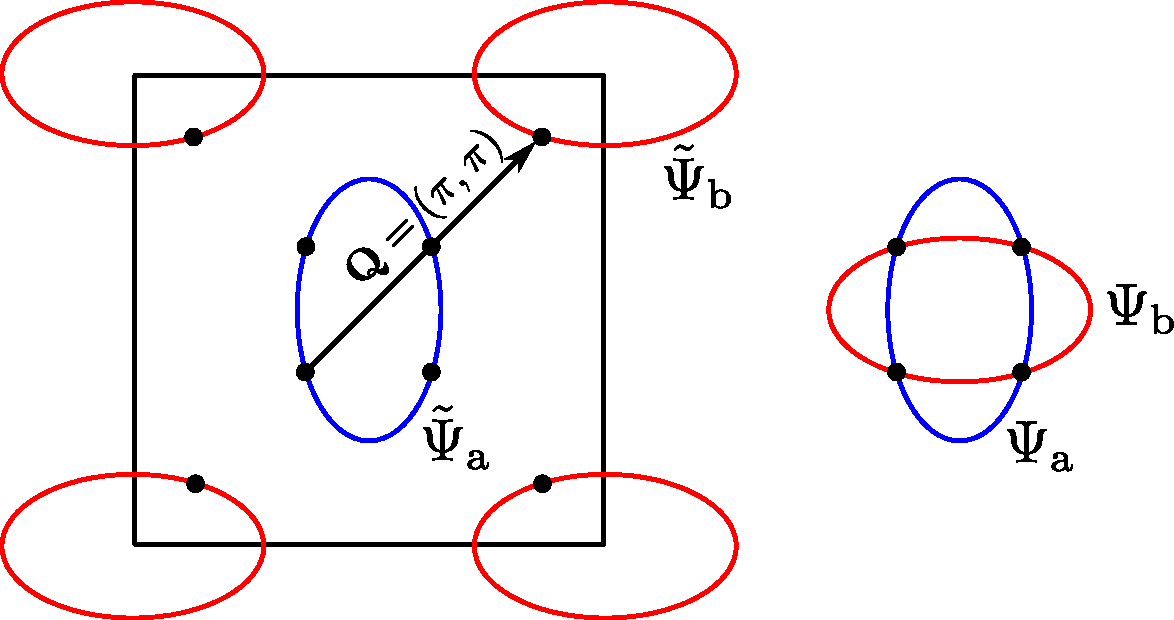
\includegraphics[width=0.7\textwidth]{hotspots.pdf}
	\caption{
One the left hand side the Brillouin zone is depicted containing the Fermi surface of both species of fermions, $\tilde{\Psi}_{\mt{a}}$ and $\tilde{\Psi}_{\mt{b}}$.
While the fermions $\tilde{\Psi}_{\mt{a}}$ are located with an anisotropic parapolical dispersion at the origin $(0,0)$, the fermions $\tilde{\Psi}_{\mt{b}}$ are located with a $\flatfrac{\pi}{2}$-rotated anisotropic parapolical dispersion at the corners of the Brillouin zone, $(\pi,\pi)$ for example.
The vector $\vb{Q}$ connects certain points on the Fermi surface, called hotspots and represented with dots. 
As a result of this an attraction between these fermions occurs.
On the right hand side the fermions $\tilde{\Psi}_{\mt{a}}$ are shifted to the corner at $(\pi,\pi)$.
The convienence of this represantation is that the coupling between fermions and spin fluctuations is local and independent of the position.
	}
	\label{fig:hotspots}
\end{figure}
%
In comparison to a normal metals these new interaction of spin fluctuations seperates the Fermi surface in "hot" and "cold" manifolds.
Considering a point $\vb{k}$ on the Fermi surface of a $d$-dimensional system, so the fermion has zero energy.
The spin density wace connects this point to another point $\vb{k}+\vb{Q}$.
We require that this point has to be also on the Fermi surface, which is our second constraints.
Both contraints yield a $d-2$-dimension manifold for a $d$-dimensional system.
In the case of $d=2$ the "hot" manifold is called a hot-spot.
Another visualization of "hot" manifolds offers the magnetic Brillouin zone spanned by the vector $\vb{Q}$.
The intersections of the magnetic Brilouin zone and the Fermi surface are eauivalent to the "hot" manifolds.

In our investigated model the fermions are considered as free up to the interaction with the spin fluctuations.
We assume two species of fermions, $\tilde{\Psi}_{\mt{a}}$ and $\tilde{\Psi}_{\mt{b}}$, with an anisotropic parabolic dispersion, as suggested in \cite{Patel&Sachdev} and depicted on the left hand side in figure \ref{fig:hotspots}.
This isn't a discrepancy to our previous constraint, assuming one fermion since both species of fermions are electrons and differ only in their dispersion.
The fermions $\tilde{\Psi}_{\mt{a}}$ and $\tilde{\Psi}_{\mt{b}}$ are located on an ellipse around the origin $(0,0)$ and $(\pi,\pi)$, respectivily.
Both ellipses are seperated by the vector $\vb{Q} = (\pi,\pi)$ and rotated by $\flatfrac{\pi}{2}$ to each other.
For achieving a continuum theory the ellipse centered around $(\pi,\pi)$ is shifted by the vector $\vb{Q}$ to the origin.
Therefore new fermionic fields, $\tilde{\Psi}_{\mt{a}}(\vb{r}) = \Psi_{\mt{a}}(\vb{r})$ and $\tilde{\Psi}_{\mt{b}}(\vb{r}) = \Psi_{\mt{b}}(\vb{r}) \exp(i\vb{Q}\vb{r})$, are introduced.
The new dispersion of the fermions $\Psi_{\mt{a}}(\vb{r})$ and $\Psi_{\mt{b}}(\vb{r})$ is depicted on the right hand side in figure \ref{fig:hotspots}
The enormous advantage is that the coupling between the fermions caused by spin density waves is local and indipendent of the position.
In reciprocal space, the free continuum Hamiltonian of the fermions $\Psi_{\mt{a}}(\vb{r})$ and $\Psi_{\mt{b}}(\vb{r})$ is given by
%
\begin{align}
	\mt{H}_{\Psi} &= 
	 	\int_{\vb{k}}\,
	 	\bigg[
	 		\epsilon_{\mt{a}}(\vb{k})
	 		\psi_{\mt{a}}^{\dag}(\vb{k},\tau)
	 		\psi_{\mt{a}}(\vb{k},\tau)
	 		+
	 		\epsilon_{\mt{b}}(\vb{k})
	 		\psi_{\mt{b}}^{\dag}(\vb{k},\tau)
	 		\psi_{\mt{b}}(\vb{k},\tau)
	 	\bigg],
	 \label{eq:Hamiltonian electrons}
\end{align}
%
where the intergal is extendsed over the first Brillouin zone and $\epsilon_{\mt{a}}(\vb{k})$ and $\epsilon_{\mt{b}}(\vb{k})$ are the anisotropic parabolical dispersions, corresponding to the fermion species a and b, given by
%
\begin{align}
	\epsilon_{\mt{a}}(\vb{k}) = \frac{k_{x}^{2}}{2m_{1}} + \frac{k_{y}^{2}}{2m_{2}} - \mu_{0}
	\qq{and}
	\epsilon_{\mt{a}}(\vb{k}) = \frac{p_{x}^{2}}{2m_{2}} + \frac{p_{y}^{2}}{2m_{1}} - \mu_{0},
	\label{eq:dispersion relations}
\end{align}
%
where $\mu_{0}$ is the chemical potential.
%
%
\section{Momentum Conservation in the Spin-Fermion-Model and the Consequence of Umklapp Scattering}
\label{sec:umklapp scattering}
%
%
In a low-energy theory, our investigated 2D-model is described by the continuum Hamiltonian $\mt{H}_{\Psi}$ for free fermions on the Fermi surface, the effective Hamiltonian $\mt{H}_{\Phi}$ for spin fluctuations and by the interaction Hamiltonian $\mt{H}_{\Psi\Phi}$ between both.
At the quantum phase transition the control parameter $r$ in \eqref{eq:Hamiltonian spin fluctuation} is zero, due to $r = \xi^{-2}$ and the correlation length $\xi$ diverges.
Thus we set $r = 0$ in the Hamiltonian $\mt{H}_{\Phi}$.
The obtained model Hamiltonian is therefore given by $\mt{H} = \mt{H}_{\Psi} + \mt{H}_{\Phi} + \mt{H}_{\Psi\Phi}$.
Our further appraoch is to prove the conservation of momentum and current for this model Hamiltonian.
After we introduce a pertubation Hamiltonian for considering umklapp scattering.
Because of this pertubation the momentum isn't anymore a conserved quantity. 
This and the consequences for the current are discussed.

A physical quantity is conserved, if its time derivative vanishes.
In quantum mechanics the time derivative is given by Heisenberg equation of motion, $\dot{\mt{A}}(t) = i\comm{\mt{H}}{\mt{A}(t)}_{-}$, where $\mt{A}(t)$ is an arbitrary operator and its partial time derivative is assumed to be zero.
The momentum operator is given by 
%
\begin{align}
	\mt{P}_{j} &= \int_{\vb{k}}\, 
		k_{j}\bigg[
	 		\Psi_{\mt{a}}^{\dag}(\vb{k},\tau) \Psi_{\mt{a}}(\vb{k},\tau)
	 		+
	 		\Psi_{\mt{b}}^{\dag}(\vb{k},\tau) \Psi_{\mt{b}}(\vb{k},\tau)
	 		-
	 		\pi_{\mu}(\vb{k},\tau) \Phi_{\mu}(-\vb{k},\tau)
		\bigg],
		\label{eq:momentum operator}
\end{align}
%
where the spatial direction is indicated by $j$, the integral is extended over the first Brillouin zone and the sum over $\mu$ is implied in the last term.
The energy-momentum-tensor, as suggested in \cite{Iliev}, is used for the computation.
Further the x-component of current operator is given by
%
\begin{align}
	\mt{J}_{\mt{x}} &= - \int_{\vb{k}}\, \bigg[
		\frac{k_{\mt{x}}}{m_{1}} \Psi_{\mt{a}}^{\dag}(\vb{k},\tau) \Psi_{\mt{a}}(\vb{k},\tau)
		+ 
		\frac{k_{\mt{x}}}{m_{2}} \Psi_{\mt{b}}^{\dag}(\vb{k},\tau) \Psi_{\mt{b}}(\vb{k},\tau)
	\bigg],
	\label{eq:current operator}
\end{align}
%
where the integral is extended over the first Brillouin zone
The y-component of the current operator is yielded by changing the index x to y and interchanging the index a and b of the fermionic field operators.
Now, the time derivative of both quantities is computed by using the basic bosonic and fermionic commutator relations.
An explicite calculation is represented in the appendix \ref{app:conservation calculation}.
This yields a vanishing time derivative for the the momentum,
%
\begin{align}
	\dot{\mt{P}}_{j} = 0,
	\label{eq:time derivative momentum}
\end{align}
%
and the following expression for the x-component of the current
%
\begin{align}
	\dot{\mt{J}}_{x} = \lambda
		\sum\limits_{\mu} \int_{\vb{k}} \int_{\vb{q}}\,
		\Phi_{\mu}(\vb{k}-\vb{q},\tau)
		\Big[
			&\Big(\frac{q_{\mt{x}}}{m_{1}} - \frac{k_{\mt{x}}}{m_{2}}\Big)
			\Psi_{\mt{b}}^{\dag}(\vb{k},\tau) \cdot \sigma_{\mu} \cdot \Psi_{\mt{a}}(\vb{q},\tau)
			\notag \\+
			&\Big(\frac{q_{\mt{x}}}{m_{2}} - \frac{k_{\mt{x}}}{m_{1}}\Big)
			\Psi_{\mt{a}}^{\dag}(\vb{k},\tau) \cdot \sigma_{\mu} \cdot \Psi_{\mt{b}}(\vb{q},\tau)
		\Big].
		\label{eq:time derivative current}
\end{align}
%
The y-component of the current is obtained by changing again the index x to y and interchanging the index a and b of the fermionic field operators.
The physical interpretation of the obtained results is that momentum is a conserved quantity and current is an unconserved quantity in the spin-fermion-model, described by the Hamiltonian H.
The Hamiltonian is further invariant with respect to time reversal symmtry and a finite overlap is possessed between both quantities.
Infinity is obtained for the static electrical conductivity in comparsion with the discussion of the previous chapter.
A finite conductivity is only obtained by broken translation symmetry.
This is equivalent to an unconserved momentum.
Therefore, the model Hamiltonian H is pertubated by umklapp scattering via the Hamiltonian
%
\begin{align}
	\mt{H}_{\mt{umklapp}} = \sum\limits_{\mu, \vb{G}} \mt{J}_{\vb{G}}
		\int_{\vb{k}}\, \Phi_{\mu}(\vb{k},\tau) \Phi_{\mu}(-\vb{k}+\vb{G},\tau),
	\label{eq:Hamiltonian umklapp scattering}
\end{align}
%
where the integral extends over the first Brillouin zone and the sum over $\vb{G}$ included all reciprocal lattice vectors.
The quantity $\mt{J}_{\vb{G}}$ is a coupling constant depending on reciprocal lattice vectors.
It is assumed that the coupling constant is decreasing fast to zero in the limit $|\vb{G}| \to \infty$.
The time derivative of the momentum is given by
%
\begin{align}
	\dot{\mt{P}}_{j}(\tau) = i \sum\limits_{\vb{G}} \mt{J}_{\vb{G}} \int_{\vb{k}} G_{j} \Phi_{\mu}(\vb{k},\tau) \Phi_{\mu}(-\vb{k} - \vb{G},\tau)
	\label{eq:time derivative momentum finite}
\end{align}
%
with respect to the new model Hamiltonian $\mt{H}' = \mt{H} + \mt{H}_{\mt{umklapp}}$.
The time derivative of the current is persisted, since the current and pertubation Hamiltonian depends on fermionic and on bosonic field operators, respectivily.
The commutator is trivially zero between both field operators.
The static electrical conductivity is become finite due to the unconserved momentum.
In the next chapter, the static electrical conductivity is explicitely computed using diagrammatic pertubation theory.














